%! TEX program = xelatex
%! TEX root = ../root.tex

\section{实验原理}
\subsection{Data Line设计}
实现Cache的最基本单元就是Data Line,在本次实验中Data Line含有与LRU替换策略有关的recent位,与替换与读写策略有关的Vaild位和Dirty位,还有数据相关的Tag位与Data位,基本结构显示如下\\

\begin{tabular}{|c|c|c|c|c|}
    \hline
    recent(1bit) & Valid(1bit) & Dirty(1bit) & Tag(23bits) & Data \\
    \hline
\end{tabular} \\

了解完Data Line的结构之后,我们就需要对Data Line中的Data结构进行分析,在本次实验中,一共有64个元素,二路主关联将64个数据分为两组,$64 \div 2 = 32 = 2^5$
所以索引的位数是5位,又由于我们需要实现三种load/store指令,所以这就要求此Cache是字节寻址的,这就意味着需要有2位的byte address(1 word等于$4 = 2 ^ 2$bytes)。 
综上所述,一个元素的结构如下:

\begin{tabular}{|c|c|c|c|}
    \hline
    Tag(23bits) & Index(5bits) & Word(2bits) & Byte(2bits) \\
    \hline
\end{tabular} \\

通过上述结构的说明,我们就能根据分析出地址各部分的含义 \\

\subsection{Cache Mode}
本次实验主要采用双路主关联,一次内存的存取会涉及到两个数据块,通过同时对比两个数据块的Tag值确定是否命中,具体的结构图如下所示:

\begin{figure}[H] %H为当前位置,!htb为忽略美学标准,htbp为浮动图形
    \centering %图片居中
    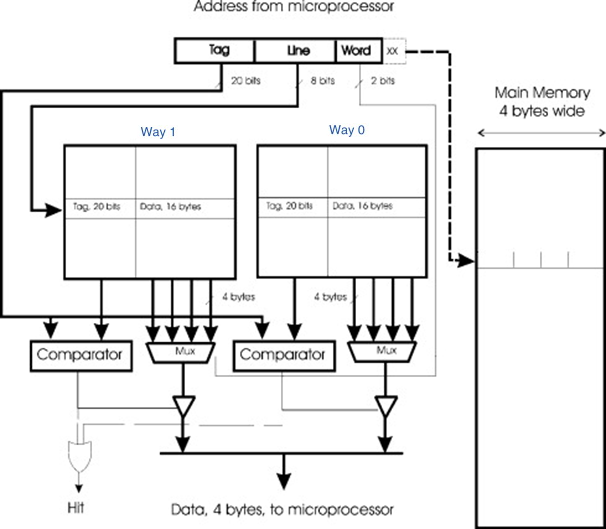
\includegraphics[width=1.0\textwidth]{figs/CacheStruct.png} %插入图片,[]中设置图片大小,{}中是图片文件名
    \caption{Cache结构} %最终文档中希望显示的图片标题
    \label{Fig.1} %用于文内引用的标签
\end{figure}

通过同时比较两个数据块是否命中,来确定整个Cache的此次读写是否命中,所以整个Cache的命中信号就可以表示为两个子部分的hit信号的并。

\subparagraph{Write Back} 本次实验中实现的是Write Back策略,
也即修改Cache的内容后,Cache并不会立即更新内存中的内容,而是等到这个Cache Line因为某种原因需要从Cache中移除时,Cache才会更新内存中的数据。
此策略在本次实验中通过Dirty位与Valid位进行实现,对缓存中的valid为1(也即有效数据)的数据进行修改之后,需要将Dirty位置为1,并不直接写入内存,
而当此块需要被替换时,才将Valid为1且Dirty为1的数据块写入内存,并且Valid位与Dirty位重新置位。同时,为了对于整个Cache的Dirty信号与Valid信号,
我们只需要将其置为下次需要被替换的Data Line的Dirty位与Valid位。

\subparagraph{Write Allocate} 本次实验中实现了Write Allocate。
Write Allocate是用于实现Write miss之后的处理,如果在写失效之后直接将需要写入的内容写入内存,那么这是no allocate的做法,而我们在此实验中是
把要写的地址所在的块先从main memory调入cache中,然后写cache,这一过程同样依赖于Valid位与Dirty位,但此过程还涉及到替换策略,我们需要决定哪一块
实验被新读入的数据块给替换掉的。

\subparagraph{LRU策略} 本次实验中用到的替换策略是LRU策略,并且由于此Cache仅是二路主关联,所以我们可以只用一位来实现这一策略,但我们读写两个数据块之一时
我们就将它的recent位置为1,并且将另一块的recent位置为0,这就可以表明最近访问的是recent位为1的那一块数据,替换的时候仅需检查recent位即可。

\subsection{源代码}
综合上述设计思想,我们组得设计代码与注释如下:

\begin{lstlisting}[language = {verilog}]
// | ----------- address 32 ----------- |
// | 31   9 | 8     4 | 3    2 | 1    0 |
// | tag 23 | index 5 | word 2 | byte 2 |

module cache (
    input wire clk,         // clock
    input wire rst,         // reset
    input wire [ADDR_BITS-1:0] addr,  // address
    input wire load,                  //  read refreshes recent bit
    input wire store,                 // set valid to 1 and reset dirty to 0
    input wire edit,                  // set dirty to 1
    input wire invalid,               // reset valid to 0
    input wire [2:0] u_b_h_w,         // select signed or not & data width
                            // please refer to definition of LB, LH, LW, LBU, LHU in RV32I Instruction Set  
    input wire [31:0] din,            // data write in
    output reg hit = 0,               // hit or not
    output reg [31:0] dout = 0,       // data read out
    output reg valid = 0,             // valid bit
    output reg dirty = 0,             // dirty bit
    output reg [TAG_BITS-1:0] tag = 0 // tag bits
    );

    `include "addr_define.vh"

    wire [31:0] word1, word2;
    wire [15:0] half_word1, half_word2;
    wire [7:0]  byte1, byte2;
    wire recent1, recent2, valid1, valid2, dirty1, dirty2;
    wire [TAG_BITS-1:0] tag1, tag2;
    wire hit1, hit2;

    //ELEMENT_NUM = 64, 一个Line有4个WORD
    reg [ELEMENT_NUM-1:0] inner_recent = 0;
    reg [ELEMENT_NUM-1:0] inner_valid = 0;
    reg [ELEMENT_NUM-1:0] inner_dirty = 0;
    //总共64个元素的tag数组
    reg [TAG_BITS-1:0] inner_tag [0:ELEMENT_NUM-1];
    // 64 elements, 2 ways set associative => 32 sets
    reg [31:0] inner_data [0:ELEMENT_NUM*ELEMENT_WORDS-1];

    // initialize tag and data with 0
    integer i;
    initial begin
        for (i = 0; i < ELEMENT_NUM; i = i + 1)
            inner_tag[i] = 23'b0;

        for (i = 0; i < ELEMENT_NUM*ELEMENT_WORDS; i = i + 1)
            inner_data[i] = 32'b0;
    end

    // the bits in an input address:
    wire [TAG_BITS-1:0] addr_tag;
    wire [SET_INDEX_WIDTH-1:0] addr_index;            // idx of set
    wire [ELEMENT_INDEX_WIDTH-1:0] addr_element1; 
    wire [ELEMENT_INDEX_WIDTH-1:0] addr_element2;     // idx of element
    wire [ELEMENT_INDEX_WIDTH+ELEMENT_WORDS_WIDTH-1:0] addr_word1;
    wire [ELEMENT_INDEX_WIDTH+ELEMENT_WORDS_WIDTH-1:0] addr_word2; // element index + word index

    assign addr_tag = addr[31:9];                   //need to fill in
    //index = set number, 32 = 2 ^ 5
    assign addr_index = addr[8:4];                  //need to fill in
    //根据结构赋值
    assign addr_element1 = {addr_index, 1'b0};
    assign addr_element2 = {addr_index, 1'b1};      //need to fill in
    assign addr_word1 = {addr_element1, addr[ELEMENT_WORDS_WIDTH+WORD_BYTES_WIDTH-1:WORD_BYTES_WIDTH]};
    assign addr_word2 = {addr_element2, addr[ELEMENT_WORDS_WIDTH+WORD_BYTES_WIDTH-1:WORD_BYTES_WIDTH]};           //need to fill in

    //与数据类型有关的赋值
    assign word1 = inner_data[addr_word1];
    assign word2 = inner_data[addr_word2];          //need to fill in
    assign half_word1 = addr[1] ? word1[31:16] : word1[15:0];
    assign half_word2 = addr[1] ? word2[31:16] : word2[15:0];     //need to fill in
    assign byte1      = addr[1] ?
                        addr[0] ? word1[31:24] : word1[23:16] :
                        addr[0] ? word1[15:8] :  word1[7:0]   ;
    assign byte2      = addr[1] ?
                        addr[0] ? word2[31:24] : word2[23:16] :
                        addr[0] ? word2[15:8] :  word2[7:0]   ;               //need to fill in

    assign recent1 = inner_recent[addr_element1];
    assign recent2 = inner_recent[addr_element2];              //need to fill in
    assign valid1 = inner_valid[addr_element1];
    assign valid2 = inner_valid[addr_element2];               //need to fill in
    assign dirty1 = inner_dirty[addr_element1];
    assign dirty2 = inner_dirty[addr_element2];               //need to fill in
    assign tag1 = inner_tag[addr_element1];
    assign tag2 = inner_tag[addr_element2];                 //need to fill in

    assign hit1 = valid1 & (tag1 == addr_tag);
    assign hit2 = valid2 & (tag2 == addr_tag);                 //need to fill in

    always @ (posedge clk) begin
        valid <= recent1 ? valid2 : valid1;
        dirty <= recent2 ? dirty1 : dirty2;    //need to fill in
        tag <= hit1 ? tag1 :
                hit2 ? tag2 : 0;                //need to fill in
        hit <= hit1 | hit2;                    //need to fill in
        
        // read $ with load==0 means moving data from $ to mem
        // no need to update recent bit
        // otherwise the refresh process will be affected
        if (load) begin
            if (hit1) begin
                dout <=
                    u_b_h_w[1] ? word1 :
                    u_b_h_w[0] ? {u_b_h_w[2] ? 16'b0 : {16{half_word1[15]}}, half_word1} :
                    {u_b_h_w[2] ? 24'b0 : {24{byte1[7]}}, byte1};
                
                // inner_recent will be refreshed only on r/w hit
                // (including the r/w hit after miss and replacement)
                inner_recent[addr_element1] <= 1'b1;
                inner_recent[addr_element2] <= 1'b0;
            end
            else if (hit2) begin
                dout <=
                    u_b_h_w[1] ? word2 :
                    u_b_h_w[0] ? {u_b_h_w[2] ? 16'b0 : {16{half_word2[15]}}, half_word2} :
                    {u_b_h_w[2] ? 24'b0 : {24{byte1[7]}}, byte2};
                
                // inner_recent will be refreshed only on r/w hit
                // (including the r/w hit after miss and replacement)
                inner_recent[addr_element1] <= 1'b0;
                inner_recent[addr_element2] <= 1'b1;    //need to fill in
            end
        end
        else dout <= inner_data[ recent1 ? addr_word2 : addr_word1 ];

        if (edit) begin
            if (hit1) begin
                inner_data[addr_word1] <= 
                    u_b_h_w[1] ?        // word?
                        din
                    :
                        u_b_h_w[0] ?    // half word?
                            addr[1] ?       // upper / lower?
                                {din[15:0], word1[15:0]} 
                            :
                                {word1[31:16], din[15:0]} 
                        :   // byte
                            addr[1] ?
                                addr[0] ?
                                    {din[7:0], word1[23:0]}   // 11
                                :
                                    {word1[31:24], din[7:0], word1[15:0]} // 10
                            :
                                addr[0] ?
                                    {word1[31:16], din[7:0], word1[7:0]}   // 01
                                :
                                    {word1[31:8], din[7:0]} // 00
                ;
                inner_dirty[addr_element1] <= 1'b1;
                inner_recent[addr_element1] <= 1'b1;
                inner_recent[addr_element2] <= 1'b0;
            end
            else if (hit2) begin
            //need to fill in
                inner_data[addr_word2] <= 
                    u_b_h_w[1] ?        // word?
                        din
                    :
                        u_b_h_w[0] ?    // half word?
                            addr[1] ?       // upper / lower?
                                {din[15:0], word2[15:0]} 
                            :
                                {word2[31:16], din[15:0]} 
                        :   // byte
                            addr[1] ?
                                addr[0] ?
                                    {din[7:0], word2[23:0]}   // 11
                                :
                                    {word2[31:24], din[7:0], word2[15:0]} // 10
                            :
                                addr[0] ?
                                    {word2[31:16], din[7:0], word2[7:0]}   // 01
                                :
                                    {word2[31:8], din[7:0]} // 00
                ;
                inner_dirty[addr_element2] <= 1'b1;
                inner_recent[addr_element2] <= 1'b1;
                inner_recent[addr_element1] <= 1'b0;
                    
            end
        end

        if (store) begin
            if (recent1) begin  // replace 2
                inner_data[addr_word2] <= din;
                inner_valid[addr_element2] <= 1'b1;
                inner_dirty[addr_element2] <= 1'b0;
                inner_tag[addr_element2] <= addr_tag;
            end else begin
                // recent2 == 1 => replace 1
                // recent2 == 0 => no data in this set, place to 1
                //need to fill in
                inner_data[addr_word1] <= din;
                inner_valid[addr_element1] <= 1'b1;
                inner_dirty[addr_element1] <= 1'b0;
                inner_tag[addr_element1] <= addr_tag;
            end
        end

        // not used currently, can be used to reset the cache.
        if (invalid) begin
            inner_recent[addr_element1] <= 1'b0;
            inner_recent[addr_element2] <= 1'b0;
            inner_valid[addr_element1] <= 1'b0;
            inner_valid[addr_element2] <= 1'b0;
            inner_dirty[addr_element1] <= 1'b0;
            inner_dirty[addr_element2] <= 1'b0;
        end
    end

endmodule    
\end{lstlisting}